\subsection{Package com::sirius::sequenziatore::server::presenter}
\begin{figure}[H] \centering 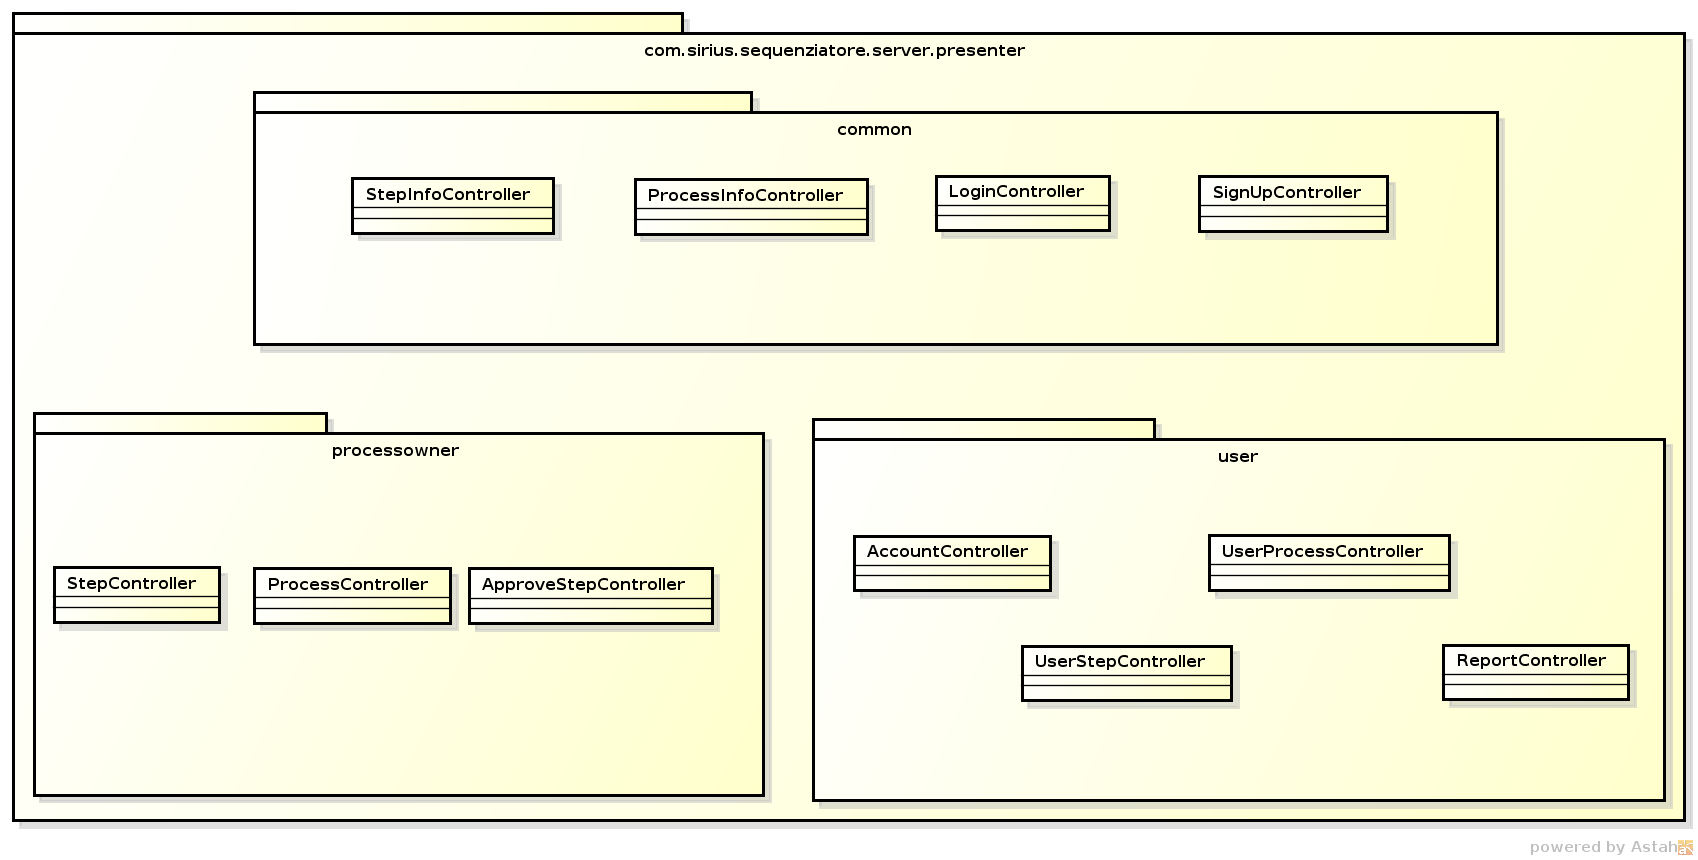
\includegraphics[width=%
\textwidth]
{./pack/ClassiServerSoloPresenter.png} \caption{Diagramma presenter server}
\end{figure}
\subsubsection{Package com::sirius::sequenziatore::server::presenter::common}
Questo \textit{package} contiene le classi che effettuano operazioni comuni tra \textit{Process Owner} e Utenti.
\paragraph{LoginController}
	\begin{itemize}
		\item \textbf{Nome:} \texttt{LoginController};
		\item \textbf{Package:} com::sirius::sequenziatore::server::presenter::common
		\item \textbf{Descrizione:} Classe che permette la gestione della login di un utente, controllando che i dati inseriti riferiscano a un utente correttamente iscritto al sistema, ponendo attenzione se esso sia un \textit{process owner} o un utente normale;
		\item \textbf{Relazione con altre componenti:} la classe invoca i metodi della classe:
		\begin{itemize}
			\item com::sirius::sequenziatore::server::dao::IDataAccessObject;
		\end{itemize}
	\end{itemize}
	
\paragraph{SignUpConroller}
	\begin{itemize}
		\item \textbf{Nome:} \texttt{SignUpController};
		\item \textbf{Package:} com::sirius::sequenziatore::server::presenter::common
		\item \textbf{Descrizione:} Classe che permette la gestione della registrazione di un nuovo utente nel sistema, nonostante la correttezza dei dati inseriti venga controllata dalla parte client, per sicurezza verrà effettuato un nuovo controllo anche sulla parte server prima di inserire ' utente nel sistema;
		\item \textbf{Relazione con altre componenti:} la classe invoca i metodi della classe:
		\begin{itemize}
			\item com::sirius::sequenziatore::server::dao::IDataAccessObject;
		\end{itemize}
	\end{itemize}
	
\paragraph{StepInfoController}
	\begin{itemize}
		\item \textbf{Nome:} \texttt{StepInfoController};
		\item \textbf{Package:} com::sirius::sequenziatore::server::presenter::common
		\item \textbf{Descrizione:} Classe che permette la gestione della registrazione di un nuovo utente nel sistema, nonostante la correttezza dei dati inseriti venga controllata dalla parte client, per sicurezza verrà effettuato un nuovo controllo anche sulla parte server prima di inserire ' utente nel sistema;
		\item \textbf{Relazione con altre componenti:} la classe invoca i metodi della classe:
		\begin{itemize}
			\item com::sirius::sequenziatore::server::dao::IDataAccessObject;
		\end{itemize}
	\end{itemize}
\paragraph{ProcessInfoController}
	\begin{itemize}
		\item \textbf{Nome:} \texttt{ProcessInfoController};
		\item \textbf{Package:} com::sirius::sequenziatore::server::presenter::common
		\item \textbf{Descrizione:} Classe che permette la gestione della registrazione di un nuovo utente nel sistema, nonostante la correttezza dei dati inseriti venga controllata dalla parte client, per sicurezza verrà effettuato un nuovo controllo anche sulla parte server prima di inserire ' utente nel sistema;
		\item \textbf{Relazione con altre componenti:} la classe invoca i metodi della classe:
		\begin{itemize}
			\item com::sirius::sequenziatore::server::dao::IDataAccessObject;
		\end{itemize}
	\end{itemize}

